% !TeX root = ../alda_g17.tex
\setcounter{chapter}{1}
\chapter{Metodología}

% ============================================================
\section{Análisis de los Datos}
% ============================================================

El sistema opera principalmente sobre datos de video RGB en tiempo real
capturados por una cámara convencional. A continuación se presenta el
análisis de los datasets de referencia utilizados para la evaluación del
desempeño, así como las características de los datos que maneja cada
módulo del proyecto.

\subsection{Datasets de Referencia}

Para la evaluación y benchmarking del sistema se utilizarán datasets
públicos consolidados en el campo de estimación de pose humana. La
elección de estos conjuntos de datos se justifica por su amplia adopción
en la literatura científica y su compatibilidad con el modelo MediaPipe
Pose. \cite{Bazarevskyetal2020, 10.1007/978-3-319-10602-1_48}

\begin{table}[h!]
\centering
\label{tab:datasets}
\renewcommand{\arraystretch}{1.3}
\begin{tabularx}{\textwidth}{
    >{\bfseries}p{3.5cm}
    X
    X
    X
    X
}
\toprule
\textbf{Dataset} &
\textbf{Tipo} &
\textbf{Imágenes / Videos} &
\textbf{Landmarks} &
\textbf{Uso en el proyecto} \\
\midrule
COCO Keypoints &
  Imágenes estáticas RGB &
  328K imágenes, 2.5M instancias &
  17 keypoints &
  Benchmark de referencia para evaluar precisión de MediaPipe Pose \\
\midrule
LSP &
  Imágenes RGB de deporte &
  2000 imágenes &
  14 keypoints &
  Validación del cálculo angular en poses con alta variabilidad \\
\bottomrule
\end{tabularx}
\caption{Datasets de referencia para evaluación del sistema.}
\end{table}

\subsection{Análisis de Datos por Módulo}

Cada módulo del sistema procesa un tipo de dato diferente. La siguiente
tabla detalla las características de los datos de entrada, las propiedades
relevantes y el preprocesamiento necesario en cada etapa del pipeline.

\begin{table}[H]
\centering
\label{tab:datos_modulo}
\renewcommand{\arraystretch}{1.3}
\begin{tabularx}{\textwidth}{
    >{\bfseries}p{2.8cm}
    X
    X
    X
}
\toprule
\textbf{Módulo} &
\textbf{Tipo de dato de entrada} &
\textbf{Características clave} &
\textbf{Preprocesamiento necesario} \\
\midrule
M1. Captura &
  Frame BGR de video (uint8, 3 canales) &
  Resolución variable; posible ruido de sensor; iluminación no controlada &
  Redimensionado a 640$\times$480; conversión BGR$\to$RGB; filtro gaussiano opcional \\
\midrule
M2. MediaPipe Pose &
  Frame RGB normalizado &
  Sujeto visible; cuerpo parcialmente ocluido hasta apróximadamente un 30\% &
  Reflejo horizontal opcional (modo selfie); ajuste de
  min\_detection\_confidence $\geq$ 0.7; extracción de landmarks 11, 13, 15, 17, 19, 21 (hombro, codo, muñeca, nudillo índice, punta índice y punta pulgar derechos) \\
\midrule
M3. Ángulos &
  Landmarks 2D (float32, $x,y \in [0,1]$) &
  Coordenadas normalizadas de 7 landmarks; fluctuaciones de ±2 a ±5 px por ruido de BlazePose; distancia euclidiana entre landmarks 19 y 21 para apertura del gripper &
  Desnormalización a píxeles; filtro media móvil $w = 5$;
  verificación de visibilidad $>$ 0.5 \\
\midrule
M4. Brazo virtual &
  Tripleta de ángulos (float64, grados) &
  Valores continuos $[0°, 180°]$; posibles discontinuidades en límites angulares &
  Clipping a rango físico válido por articulación;
  interpolación lineal para suavizado extra \\
\midrule
M5. Visualización &
  Frame BGR + overlays compuestos &
  Alta variabilidad según iluminación y fondo &
  Sin preprocesamiento adicional; medición de FPS por diferencia de timestamps \\
\bottomrule
\end{tabularx}
\caption{Análisis de datos de entrada, características y preprocesamiento por módulo.}
\end{table}

\subsection{Análisis de Confiabilidad y Compatibilidad}

Se analiza la confiabilidad de las principales soluciones existentes y su
compatibilidad con los requisitos del proyecto. MediaPipe Pose (BlazePose)
ha sido validado con una diferencia de precisión
inferior al 10\% respecto a sistemas IMU de referencia en estimación de
movimientos corporales. \cite{Pauzietal2021}

En términos de compatibilidad tecnológica, el stack seleccionado
(Python + OpenCV + MediaPipe) presenta las siguientes garantías:
(a)~compatibilidad multiplataforma (Windows, Linux, macOS) sin modificación
del código; (b)~ausencia de dependencias de GPU, lo que elimina problemas
de compatibilidad de drivers; (c)~todas las librerías son de código
abierto con licencias Apache 2.0 o BSD, sin restricciones de uso
académico; y (d)~versiones estables con soporte activo a la fecha del
proyecto (2026). \cite{Bazarevskyetal2020, Lugaresietal2019, Bradski2000}

\begin{itemize}[leftmargin=1.5em]
  \item \textbf{MediaPipe Pose v0.10+:} estable desde 2022, soportado
        en Python 3.8--3.12, compatible con OpenCV 4.x. Latencia de
        inferencia $<$ 30 ms en CPU. \cite{Bazarevskyetal2020}
  \item \textbf{OpenCV v4.8+:} librería de visión computacional más
        usada globalmente, con más de 20 años de desarrollo activo y
        amplia documentación. \cite{Bradski2000}
  \item \textbf{NumPy v1.24+:} librería estándar de álgebra numérica
        en Python, prerequisito de todas las demás librerías del stack.
\end{itemize}

% ============================================================
\section{Alcance del Proyecto}
% ============================================================

El alcance del proyecto queda delimitado por los siguientes criterios:
el sistema procesa video de una sola persona visible en cámara
(single-person pose estimation), en entornos con iluminación
entre 50 y 500 lux, con el sujeto a una distancia de 1--3 metros de la
cámara. El brazo robótico virtual es una simulación 2D renderizada en
pantalla y no controla hardware físico. \cite{Vintimilla2026}

\subsection{Requerimientos}

\subsubsection*{Requerimientos Funcionales}

\begin{table}[h!]
\centering
\label{tab:req_func}
\renewcommand{\arraystretch}{1.3}
\begin{tabularx}{\textwidth}{
    >{\bfseries}p{1.1cm}
    X
    p{1.6cm}
    p{2.2cm}
}
\toprule
\textbf{ID} &
\textbf{Requerimiento} &
\textbf{Prioridad} &
\textbf{Módulo(s)} \\
\midrule
RF-01 &
  El sistema debe capturar video en tiempo real desde una cámara RGB a
  mínimo 30 FPS &
  Alta & M1 \\
\midrule
RF-02 &
  El sistema debe detectar la pose del cuerpo humano usando MediaPipe
  Pose con una confianza mínima de 0.7, extrayendo únicamente los
  landmarks 11, 13, 15, 17, 19 y 21 correspondientes al hombro, codo,
  muñeca, nudillo, punta del índice y punta del pulgar derechos &
  Alta & M2, M3 \\
\midrule
RF-03 &
  El sistema debe calcular los ángulos de hombro, codo y muñeca con un
  error máximo de $\pm$5° &
  Alta & M3 \\
\midrule
RF-04 &
  El sistema debe aplicar filtro de media móvil de ventana $w = 5$
  para suavizar los ángulos calculados &
  Media & M3 \\
\midrule
RF-05 &
  El sistema debe renderizar un brazo robótico virtual de 3 GDL
  sincronizado con el movimiento en tiempo real &
  Alta & M4 \\
\midrule
RF-06 &
  El sistema debe mostrar los ángulos articulares y las métricas de FPS
  superpuestas en el frame de video &
  Media & M5 \\
\midrule
RF-07 &
  El sistema debe exportar el video procesado a un archivo MP4 cuando
  el usuario lo requiera &
  Baja & M5 \\
\midrule
RF-08 &
  El sistema debe procesar al menos 20 FPS en hardware de CPU estándar
  (sin GPU) &
  Alta & M1, M5 \\
\midrule
RF-09 &
El sistema debe calcular la apertura del gripper como la distancia euclidiana normalizada entre la punta del índice (landmark 19) y la punta del pulgar (landmark 21), mapeada al rango [0\%, 100\%] &
Alta & M3, M4 \\
\bottomrule
\end{tabularx}
\caption{Requerimientos funcionales del sistema.}
\end{table}

\subsubsection*{Requerimientos No Funcionales}

\begin{table}[H]
\centering
\label{tab:req_nofunc}
\renewcommand{\arraystretch}{1.3}
\begin{tabularx}{\textwidth}{
    >{\bfseries}p{1.1cm}
    X
    X
}
\toprule
\textbf{ID} &
\textbf{Requerimiento} &
\textbf{Criterio de aceptación} \\
\midrule
RNF-01 &
  Rendimiento: $\geq$ 20 FPS en CPU Intel Core i5 con 8 GB RAM &
  FPS promedio medido sobre 500 frames consecutivos $\geq$ 20 \\
\midrule
RNF-02 &
  Precisión angular: error medio (MAE) $\leq$ 5° respecto a medición
  de referencia &
  MAE calculado sobre 100 poses con transportador digital de referencia \\
\midrule
RNF-03 &
  Robustez: detección estable con variaciones de iluminación entre
  50 y 500 lux &
  Tasa de detección exitosa $\geq$ 90\% en el rango de iluminación
  especificado \\
\midrule
RNF-04 &
  Portabilidad: ejecución en Windows 10+ y Ubuntu 20.04+
  sin modificaciones &
  Instalación y ejecución exitosa en las tres plataformas con el mismo
  código fuente \\
\midrule
RNF-05 &
  Usabilidad: tiempo de configuración inicial $\leq$ 10 minutos &
  Seguir la guía de instalación del README y completarla en el tiempo
  estipulado \\
\midrule
RNF-06 &
  Mantenibilidad: código estructurado en módulos independientes con
  docstrings en cada función &
  Cobertura de docstrings $\geq$ 80\% verificada con pydocstyle por ejemplo. \\
\bottomrule
\end{tabularx}
\caption{Requerimientos no funcionales del sistema.}
\end{table}

\subsection{Recursos a Utilizar}

\subsubsection*{Hardware}

\begin{table}[H]
\centering
\label{tab:hardware}
\renewcommand{\arraystretch}{1.3}
\begin{tabularx}{\textwidth}{
    >{\bfseries}p{3cm}
    X
    X
}
\toprule
\textbf{Recurso} &
\textbf{Especificación mínima} &
\textbf{Justificación} \\
\midrule
Computador Laptop &
  Intel Core i5 (8ª gen+) o AMD Ryzen 5; 8 GB RAM;
  Windows 10 / Ubuntu 20.04 &
  MediaPipe Pose opera en CPU sin GPU; la especificación mínima garantiza
  $\geq$ 20 FPS \\
\midrule
Cámara web (webcam) &
  Resolución mínima 640$\times$480 @ 30 FPS; interfaz USB 2.0 o integrada &
  Compatible con cv2.VideoCapture(0); cualquier cámara reconocida
  por el SO \\
\midrule
Espacio en disco &
  500 MB libres para entorno virtual y dependencias &
  Python + OpenCV + MediaPipe + dependencias con tamaño aproximado de 450 MB \\
\midrule
Conexión a internet &
  Necesaria solo para instalación inicial de paquetes pip &
  Requerida en Sprint 2 para descargar modelos BlazePose (mas o menos 25 MB) \\
\bottomrule
\end{tabularx}
\caption{Recursos de hardware requeridos.}
\end{table}

\subsubsection*{Software y Librerías}

\begin{table}[h!]
\centering
\label{tab:software}
\renewcommand{\arraystretch}{1.3}
\begin{tabularx}{\textwidth}{
    >{\bfseries}p{3cm}
    p{2cm}
    p{2.2cm}
    X
}
\toprule
\textbf{Librería / Herramienta} &
\textbf{Versión} &
\textbf{Licencia} &
\textbf{Rol en el proyecto} \\
\midrule
Python        & 3.10+  & PSF         & Lenguaje principal de implementación \\
\midrule
OpenCV (cv2)  & 4.8+   & Apache 2.0  & Captura, preprocesamiento, renderizado y visualización (M1, M4, M5) \cite{Bradski2000} \\
\midrule
MediaPipe     & 0.10+  & Apache 2.0  & Detección de pose BlazePose; extracción de landmarks 11, 13, 15, 17, 19, 21 para ángulos articulares y apertura del gripper (M2, M3) \cite{Bazarevskyetal2020, Lugaresietal2019} \\
\midrule
NumPy         & 1.24+  & BSD         & Álgebra vectorial para cálculo angular y manejo de arrays (M3) \\
\midrule
Matplotlib    & 3.7+   & PSF         & Gráficas de evolución de ángulos articulares y métricas FPS (M5) \\
\midrule
scikit-learn  & 1.3+   & BSD         & Métricas estadísticas: MAE, correlación de Pearson (evaluación opcional) \\
\midrule
Git / GitHub  & 2.40+  & GPL / MIT   & Control de versiones y gestión del repositorio del proyecto \\
\bottomrule
\end{tabularx}
\caption{Stack de software y librerías del proyecto con versiones y licencias.}
\end{table}

\subsection{Diseño Conceptual}

El diseño conceptual del sistema se articula en torno a un pipeline de
procesamiento en tiempo real compuesto por los cinco módulos definidos en
el Sprint \#1. El flujo completo se ejecuta en un bucle principal a la
frecuencia de la cámara (30 FPS objetivo). El tiempo total de
procesamiento por frame debe ser inferior a 50 ms para garantizar el
requisito de $\geq$ 20 FPS. \cite{Bazarevskyetal2020, Bradski2000}

\subsubsection*{Arquitectura General del Pipeline}

La figura \ref{fig:pipeline} representa el flujo de datos del sistema
desde la captura hasta la visualización.

\begin{figure}[h!]
    \centering
    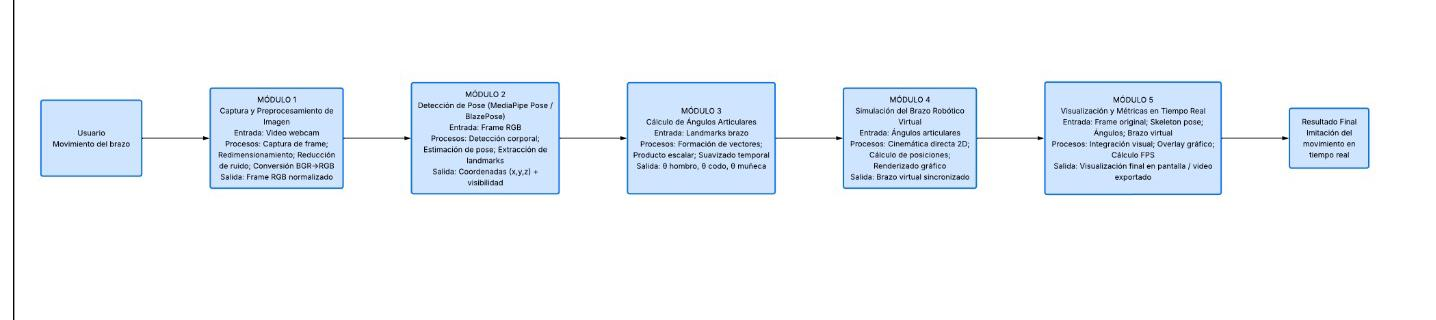
\includegraphics[width=1\textwidth]{images/diagrama_bloques.jpeg}
    \caption{Arquitectura conceptual del pipeline de procesamiento en tiempo real.}
    \label{fig:pipeline}
\end{figure}

\subsubsection*{Diseño del Módulo M3 -- Cálculo de Ángulos}

El módulo M3 implementa el cálculo de ángulos mediante la siguiente
lógica para cada articulación:

\begin{enumerate}
    \item Extraer las coordenadas 2D $(x, y)$ en píxeles de los landmarks
          proximal, central y distal de la articulación.
    \item Construir los vectores $\vec{v}_1$ (de central a proximal) y
          $\vec{v}_2$ (de central a distal).
    \item Calcular el ángulo mediante la ecuación \ref{eq:angulo_s2}:
          \begin{equation}
              \theta \;=\; \arccos\!\left(
                \frac{\vec{v}_1 \cdot \vec{v}_2}
                     {|\vec{v}_1|\,|\vec{v}_2|}
              \right)
              \label{eq:angulo_s2}
          \end{equation}
          El resultado en radianes se convierte a grados.
    \item Aplicar filtro de media móvil de ventana $w = 5$ sobre el
          historial de ángulos de la articulación.
    \item Retornar el ángulo suavizado junto con un flag de validez
          (\texttt{True} si visibilidad de todos los landmarks $>$ 0.5).
    \item Calcular la apertura del gripper: distancia euclidiana entre landmark 19 (punta índice) y landmark 21 (punta pulgar), normalizada entre un valor mínimo $d_{min}$ (pinza cerrada) y máximo $d_{max}$ (pinza abierta), expresada como porcentaje [0\%, 100\%].
\end{enumerate}

\subsubsection*{Diseño del Módulo M4 -- Cinemática Directa 2D}

El brazo robótico virtual se modela como una cadena cinemática de tres
eslabones más un efector final tipo gripper, anclada en una posición
fija de la pantalla (base). Las longitudes de eslabón son parámetros
configurables (en píxeles):

\begin{itemize}[leftmargin=1.5em]
    \item $L_{\text{hombro}} = 120$ px (eslabón 1: base $\to$
          articulación 1)
    \item $L_{\text{antebrazo}} = 100$ px (eslabón 2: articulación 1
          $\to$ articulación 2)
    \item $L_{\text{mano}} = 60$ px (eslabón 3: articulación 2
          $\to$ efector final)
    \item $L_{\text{gripper}} = 30$ px por rama (dos segmentos
          divergentes que representan la apertura de la pinza;
          el ángulo entre ellos es proporcional a
          $a_{\text{gripper}}$ calculado en M3)
\end{itemize}

Las posiciones cartesianas de cada junta se calculan mediante cinemática
directa acumulativa (ecuaciones \ref{eq:cinematica_s2}):

\begin{align}
  x_1 &= x_0 + L_{\text{hombro}}\cos(\theta_{\text{hombro}})
  \notag \\
  y_1 &= y_0 - L_{\text{hombro}}\sin(\theta_{\text{hombro}})
  \notag \\
  x_2 &= x_1 + L_{\text{antebrazo}}
               \cos(\theta_{\text{hombro}} + \theta_{\text{codo}})
  \notag \\
  y_2 &= y_1 - L_{\text{antebrazo}}
               \sin(\theta_{\text{hombro}} + \theta_{\text{codo}})
  \label{eq:cinematica_s2}
\end{align}

\subsection{Bocetos y Flujos de Pantalla}

A continuación se describen los bocetos del sistema y los flujos de
pantalla principales. Los bocetos representan la disposición visual de
la interfaz de usuario en la ventana de visualización de OpenCV.

\subsubsection*{Boceto 1 -- Pantalla Principal (Vista en tiempo real)}

La ventana principal muestra el frame de video (640$\times$480 px) con
los siguientes elementos superpuestos:

\begin{figure}[H]
    \centering
    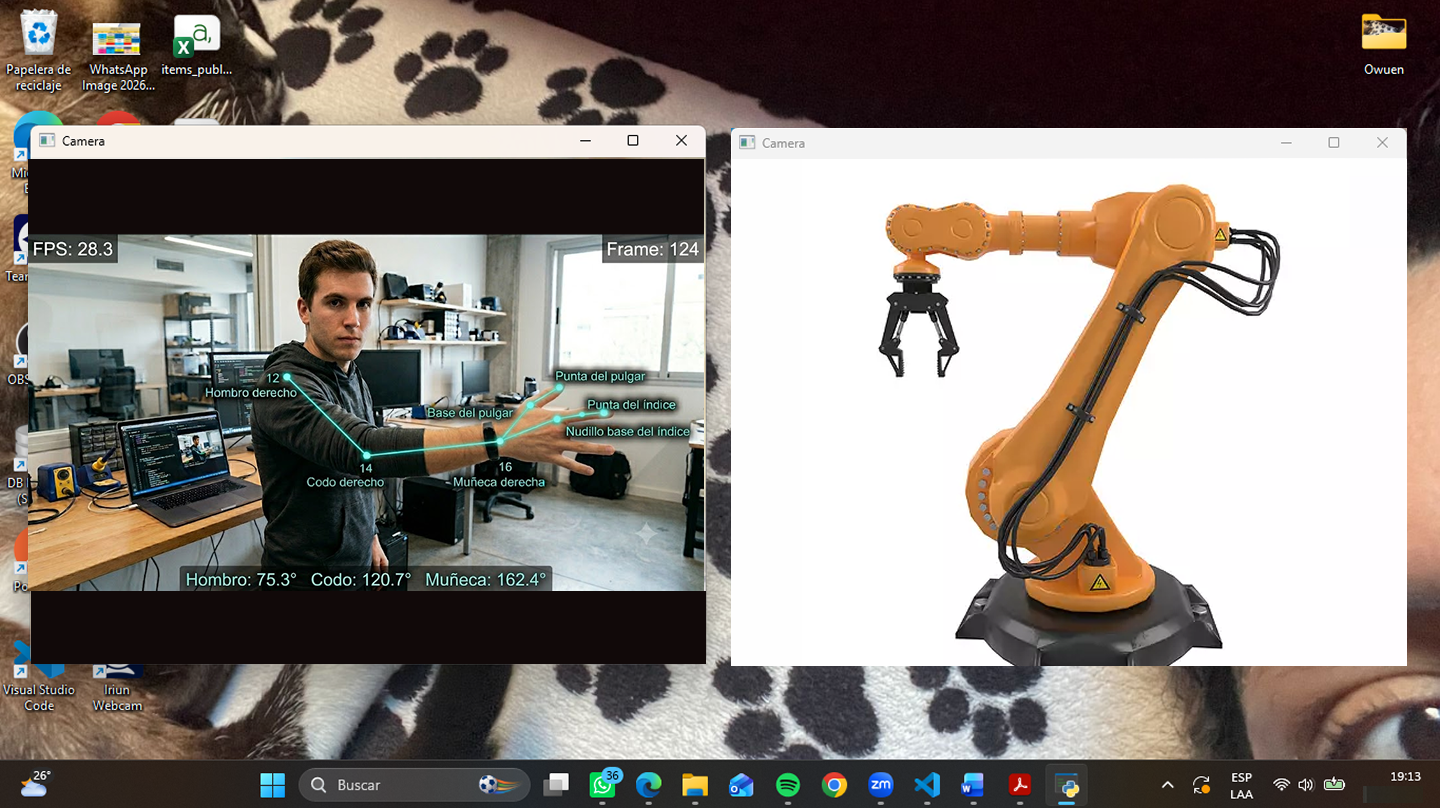
\includegraphics[width=0.75\textwidth]{images/boceto_pantalla.png}
    \caption{Boceto de la pantalla principal del sistema (ventana OpenCV en
             tiempo real). Elementos: contador FPS, número de frame,
             skeleton MediaPipe con landmarks,  brazo robótico
             virtual, ángulos articulares
             calculados en tiempo real.}
    \label{fig:boceto_pantalla}
\end{figure}

\subsubsection*{Boceto 2 -- Flujo de Pantalla del Sistema}

El flujo de interacción del usuario con el sistema sigue la secuencia
de estados de la figura \ref{fig:flujo_pantalla}.

\begin{figure}[h!]
    \centering
    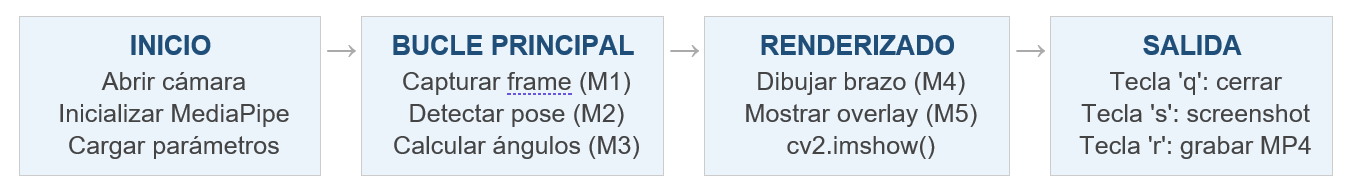
\includegraphics[width=1\textwidth]{images/flujo_pantalla.png}
    \caption{Flujo de pantalla del sistema}
    \label{fig:flujo_pantalla}
\end{figure}

% ============================================================
\section{Plan de Implementación del Proyecto}
% ============================================================

El plan de implementación sigue la metodología SCRUM con tres sprints.
El Sprint \#1 (semanas 1--2) cubrió la definición del problema. El
Sprint \#2 (semanas 3--4) cubre la metodología. El Sprint \#3
(fin del curso DIP) abarca el desarrollo completo, análisis de resultados y
conclusiones. \cite{Vintimilla2026}

\begin{table}[H]
\centering
\label{tab:plan_impl}
\renewcommand{\arraystretch}{1.3}
\begin{tabularx}{\textwidth}{
    >{\bfseries}p{1.5cm}
    p{1.6cm}
    X
    p{3.5cm}
}
\toprule
\textbf{Sprint} &
\textbf{Semanas} &
\textbf{Actividades principales} &
\textbf{Entregable} \\
\midrule
Sprint \#1 & 1--2 &
  Revisión del estado del arte (tema macro, componentes y herramientas).
  Definición del diagrama de bloques y módulos. Definición de objetivos,
  entradas y salidas por módulo. &
  Informe \#1 (Secciones 1.1--1.5) \\
\midrule
Sprint \#2 & 3--4 &
  Análisis de datos (datasets, características, preprocesamiento).
  Análisis de confiabilidad y compatibilidad. Definición de
  requerimientos, recursos, diseño conceptual y bocetos. Plan de
  implementación. &
  Informe \#2 (Sección 2) \\
\midrule
Sprint \#3 -- Fase 1 & 5--7 &
  M1: captura y preprocesamiento (cv2.VideoCapture, normalización,
  filtro gaussiano). M2: integración MediaPipe Pose y extracción de
  landmarks 11--16. M3: cálculo vectorial de ángulos con filtro media
  móvil y pruebas unitarias. Incluye cálculo de apertura del gripper por distancia euclidiana landmarks 19–21. &
  Código M1--M3 funcional + pruebas unitarias \\
\midrule
Sprint \#3 -- Fase 2 & 8--10 &
  M4: cinemática directa 2D, renderizado del brazo y simulación visual del gripper (apertura/cierre). M5:
  visualización integrada y FPS overlay. Integración de M1--M5 en
  pipeline completo. &
  Sistema integrado funcional a $\geq$ 20 FPS \\
\midrule
Sprint \#3 -- Fase 3 & 11--12 &
  Evaluación del sistema: FPS, MAE angular, robustez ante iluminación.
  Análisis estadístico con scikit-learn y gráficas con matplotlib.
  Redacción de conclusiones, recomendaciones y futuros trabajos. &
  Informes \#3 y \#4 (Secciones 3 y 4) \\
\bottomrule
\end{tabularx}
\caption{Plan de implementación del proyecto por sprint y semanas.}
\end{table}

\subsection{Gestión de Riesgos}

Se identifican los siguientes riesgos técnicos con sus planes de
mitigación:

\begin{table}[H]
\centering
\label{tab:riesgos}
\renewcommand{\arraystretch}{1.3}
\begin{tabularx}{\textwidth}{
    X
    p{2cm}
    p{1.8cm}
    X
}
\toprule
\textbf{Riesgo} &
\textbf{Probabilidad} &
\textbf{Impacto} &
\textbf{Mitigación} \\
\midrule
FPS $<$ 20 en hardware de bajo rendimiento &
  Media & Alto &
  Reducir resolución a 320$\times$240; desactivar skeleton completo;
  usar MoveNet como fallback \\
\midrule
Oclusión del brazo en poses extremas &
  Alta & Medio &
  Implementar umbral de visibilidad ($>$ 0.5); mantener último ángulo
  válido cuando visibilidad es baja \\
\midrule
Ruido excesivo en landmarks por iluminación deficiente &
  Media & Medio &
  Aumentar ventana de media móvil a $w = 10$; Inversión de capital en mejorar condiciones de iluminación \\
\midrule
Incompatibilidad de versiones de librerías &
  Baja & Alto &
  Fijar versiones exactas en requirements.txt; usar entorno
  virtual Python aislado \\
\bottomrule
\end{tabularx}
\caption{Identificación de riesgos técnicos y planes de mitigación.}
\end{table}